\documentclass[a0,landscape]{a0poster}
%\documentclass[a0,draft]{a0poster}
% With the word preview in the square bracket, your poster will be a4
% size, handy for previewing or submit to x4u queue for A0. 
% with preview removed, you get a file the right size for the HP
% large-format printer. This is a bit bigger than A0, the width is 
% exactly one imperial yard.

% This is so we can have multiple columns of text side-by-side
\usepackage[utf8]{inputenc}
\usepackage{graphicx}
\usepackage{multicol}
\usepackage{helvet}
\usepackage{sectsty}
%\allsectionsfont{\usefont{OT1}{phv}{bc}{n}\selectfont}
\allsectionsfont{\sffamily} \subsubsectionfont{\sffamily\large}
\columnsep=100pt 

% This is the thickness of the black line between the columns of text
\columnseprule=3pt

% this package gives you coloured text and various other simple
% graphics hacks. 
% Details in /usr/local/teTeX/texmf/doc/generic/pstricks/*
\usepackage{pstricks}

%\psset{unit=1cm}

\usepackage{times}
\usepackage{url}

% Define names for some colours 
\newcmykcolor{Inblue}{1.00 0.37 0.00 0.00}
\newcmykcolor{Inred}{0.00 1.00 0.63 0.00}
\newrgbcolor{Inmaroon}{0.4 0.0 0.4}
\newrgbcolor{darkblue}{0.0 0.0 0.5}

% Colour used for figure captions. Change to suit your own preference
\newrgbcolor{captcolor}{0.0 .5 0.0}

\begin{document}

% This is black magic to put a title at the top of the page.
% Thanks to Mark ``the magician'' Filipiak, although I have re-done a
% lot of the code here -- hopefully it is more robust.

% Make a box 0.55* width of poster for title and names
% If your title is long, replace 0.55 with something bigger and 
% make the box for the address smaller by the same amount.
\begin{minipage}[b]{0.65\linewidth} 
\veryHuge \bf 
\textsf{Rapid rule-based machine translation between Dutch and Afrikaans}
\\[1cm]
\huge \bf Pim Otte, Francis M. Tyers,\\
\huge \rm Mendelcollege, Universitat d'Alacant
\end{minipage}
% Make box 0.35 X width of poster for address  
\begin{minipage}[b]{0.35\linewidth} 
\Large Departament de Llenguatges i Sistemes Inform\`{a}tics\\
Universitat d'Alacant\\
E-03071 Alacant\\
Spain\\
\tt{email: ftyers@prompsit.com}
\end{minipage}
%% Make box 0.05*width of poster for EU Shield graphic
%\begin{minipage}[b]{0.05\linewidth}
%\includegraphics[width=10cm]{logo_ofis_liv.pdf}
%%\includegraphics{uitlogo}
%\end{minipage}
\vspace{0.3cm}
\hrule
\vspace{0.3cm}
%\begin{minipage}[b]{\linewidth} 
%\hrule
%{\small \url{http://www.ofis-bzh.org/bzh/ressources_linguistiques/index-troerofis.php}}
%\end{minipage}
%

% This is how many columns your poster will be broken into.
\begin{multicols}{4}

% This is the width your figures will be scaled to. Change this if you 
% change the number of columns.
\newlength{\figwidth}
\setlength{\figwidth}{20cm}

% Set to half of figwidth. Used for putting two figs side by side
\newlength{\fighalfwidth}
\setlength{\fighalfwidth}{10cm}

% Can't use the figure environment within multicolumns. Set up our own 
% counter for figures.
\newcounter{figscount}

\section{Introduction}

\noindent
{\bf Dutch} is a West-Germanic language spoken by nearly 23 million people, mostly from the 
Netherlands and Flanders. {\bf Afrikaans} is spoken by at least 5 million people, mainly in 
South-Africa,but also in Namibia. Afrikaans is a variety of Dutch that originates from that 
spoken by the the Dutch colonists of the Cape Colony. In 1925 Afrikaans replaced Dutch as
an official language in South-Africa, to be the joint official language together with English.

\vspace{1.5cm}

\section{Method}

\noindent
The system is based on {\bf Apertium} (\url{http://www.apertium.org/}), a free/open-source rule-based
machine translation platform. To create the language pair we used an existing resource and created 
several new ones. \\

\begin{center}
\begin{minipage}[b]{26cm}
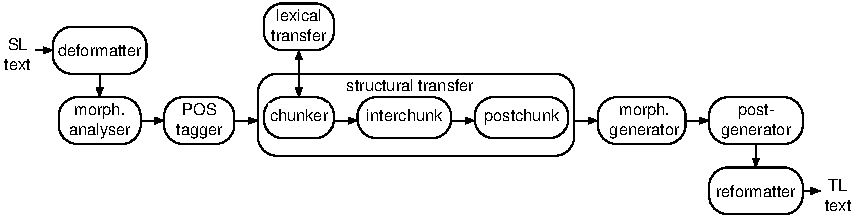
\includegraphics[width=260mm]{apertium2.pdf}
\end{minipage}\\
\textbf{Figure 4:} Modules of the Apertium translation system
\vspace{0.3cm}
\end{center}


\vspace{1.5cm}

\subsection{Existing resources}

\noindent
We reused the morphological transducer for Afrikaans, created during a currently dormant English-Afrikaans
Machine Translation project.\\

\subsection{Resources created}

\subsubsection{Dutch morphological transducer}
A new Dutch morphological transducer was created, because existing ones were unsuitable for several reasons:

\begin{itemize}
 \item Non-free license
 \item Not bidirectional
 \item Tagset different from Afrikaans transducer
\end{itemize}

\vspace{0.5cm}

\noindent
The open categories (nouns, verbs, adjectives, adverbs) for the Dutch 
morphological analyser were extracted semi-automatically from 
Wiktionary, (\url{http://www.wiktionary.org}), which has entries like \ref{fig:wikt1}
Closed categories were added by hand based on a grammar of Dutch.
\vspace{0.5cm}

\begin{figure}
\centering
\begin{tiny}
\begin{tabular}{|l|}
\hline
{\large Dutch} \\
~\\
{\bf Etymology}\\
~\\
~{\em hoofd-} (``main, head'') + {\em stad} (``city'')\\
~\\
{\bf Pronunciation}\\
~\\
{\bf Noun}\\
~\\
{\bf hoofdstad} m. ({\em pl} hoofdsteden, {\em dimin} hoofdstadje, {\em dimin pl} hoofdstadjes) \\
~\\
~~~~1. capital city \\

\hline
\end{tabular}
\end{tiny}
\caption{English language Wiktionary article for Dutch \emph{hoofdstad} `capital city' 
    {\small http://en.wiktionary.org/wiki/hoofdstad}}
\label{fig:wikt1}
\end{figure}
\vspace{0.5cm}

\noindent
The analyser has a coverage of between 87--90\% over two free corpora of Breton (Wikipedia and \emph{Bremaik}).

\subsection{Part-of-speech tagging}

\noindent
The part-of-speech tagging module for the system is based on two technologies, the first is 
Constraint Grammar, which uses linguist-written rules to disambiguate
morphologically ambiguous words based on sentence context. The second is a
bigram HMM part-of-speech tagger.

\subsubsection{Constraint grammar}

\noindent
The Breton constraint grammar has been written manually and contains 206 rules
for disambiguating Breton sentences. \\

\begin{center}
\begin{minipage}[b]{25cm}
\begin{small}
\begin{verbatim}
^Gallout/Gallout<vblex><inf>$    
^a/a<vpart><subj>$                   SELECT:194
^ran/ober<vblex><pri><p1><sg>$ 
^ober/ober<vblex><inf>$              REMOVE:205
^an/an<det><def><sp>$                REMOVE:322
^dra/tra<n><m><sg>$ 
^-se/se<adv>$
^./.<sent>$
\end{verbatim}
\end{small}
\end{minipage}\\
~\\
\textbf{Figure 6:} Morphological disambiguation with constraint grammar
\vspace{0.5cm}
\end{center}

\noindent
An extract from the constraint grammar rule set:\\

\begin{small}
\begin{verbatim}
  # ex.  "Dav e vije"
  SELECT:194 Vpart IF (1C VerbFin);

  # ex.  "Ober a ra gwestell"
  REMOVE:205 ("ober" n) IF (NOT -1 Det);

  # ex.  "An dud a zeu da Roazhon"
  REMOVE:322 VerbFin IF (0 Det) (1 NC);
\end{verbatim}
\end{small}

\subsubsection{HMM-based tagger}

\noindent
The HMM-based tagger was trained on a database dump of the Breton Wikipedia (\url{http://br.wikipedia.org}) and
chooses a single analysis where the constraint grammar does not perform a complete disambiguation.\\

\subsection{Bilingual dictionary}

\noindent
The bilingual dictionary, or transfer lexicon contains mappings between lemmas,
parts-of-speech and other tags. For example, to indicate to the transfer stage
that gender and number need to be inserted, or to indicate a change in a feature.\\

\begin{center}
\begin{minipage}[b]{26cm}
\begin{small}
\begin{verbatim}
<l>an<s n="det"/></l><r>le<s n="det"/></r><par n="sp_GDND"/>
<l>se<s n="adv"/></l><r>ci<s n="adv"/></r>
<l>tra<s n="n"/><s n="m"/></l><r>chose<s n="n"/><s n="f"/></r>
<l>gallout<s n="vblex"/></l><r>pouvoir<s n="vbmod"/></r>
<l>ober<s n="vblex"/></l><r>faire<s n="vblex"/></r>
\end{verbatim}
\end{small}
\end{minipage}\\
~\\
\textbf{Figure 7:} Extract from the bilingual dictionary
\vspace{0.3cm}
\end{center}

\subsection{Transfer rules}

\noindent
The structural transfer process is split into three parts. Rules are written in XML (see example in Figure 9).

\subsubsection{Chunker}

\noindent
Local transfer operations and chunking are performed by the first stage. The output in Figure 8 is generated by two rules.  The first takes a sequence of an infinitive verb, followed by a verbal particle and a form of 
the auxiliary \emph{ober} `to do' and outputs the infinitive verb conjugated according 
to the auxiliary. The second rule (see Figure 9) takes a sequence of determiner, followed by a noun and a 
demonstrative adverb and outputs a demonstrative determiner followed by the noun.\\

\begin{center}
\begin{minipage}[b]{26cm}
\begin{small}
\begin{verbatim}
^Verbcj<SV><vbmod><pri><p1><sg>{^pouvoir<vbmod><pri><4><5>$}$ 
^faire<SV><vblex><inf><sg>{^faire<vblex><inf>$}$ 
^det_nom<SN><f><sg>{^ce<det><dem><2><3>$ ^chose<n><2><3>$}$
^punt<sent>{^.<sent>$}$
\end{verbatim}
\end{small}
\end{minipage}\\
~\\
\textbf{Figure 8:} Output from the the first transfer stage
\vspace{0.5cm}
\end{center}
\vspace{0.2cm}

\begin{center}
\begin{minipage}[b]{25cm}
\begin{small}
\begin{verbatim}
<rule comment="REGLA: an dra-se : cette chose">
  <pattern>
    <pattern-item n="det"/>
    <pattern-item n="nom"/>
    <pattern-item n="dem"/>
  </pattern>
  <action>
    <call-macro n="f_concord2">
      <with-param pos="2"/>
      <with-param pos="1"/>
    </call-macro>
    <out>
      <chunk name="det_nom">
        <tags>
          <tag><lit-tag v="SN"/></tag>
          <tag><var n="genero"/></tag>
          <tag><var n="numero"/></tag>
        </tags>
        <lu>
          <lit v="ce"/>
          <lit-tag v="det.dem"/>
          <clip pos="1" side="tl" part="gen" link-to="2"/>
          <clip pos="1" side="tl" part="nbr" link-to="3"/>
        </lu>
        <b pos="1"/>
        <lu>
          <clip pos="2" side="tl" part="lem"/>
          <clip pos="2" side="tl" part="a_nom"/>
          <clip pos="2" side="tl" part="gen" link-to="2"/>
          <clip pos="2" side="tl" part="nbr" link-to="3"/>
        </lu>
      </chunk>
    </out>
  </action>
</rule>
\end{verbatim}
\end{small}
\end{minipage}\\
~\\
\textbf{Figure 9:} Rule to translate a demonstrative noun phrase
\vspace{0.5cm}
\end{center}
\vspace{0.2cm}

\subsubsection{Interchunk}

\noindent
The second stage of transfer, \emph{interchunk} performs global operations between chunks. For example
the insertion and concordance of a missing subject pronoun as in Figure 9.\\

\begin{center}
\begin{minipage}[b]{26cm}
\begin{small}
\begin{verbatim}
^Prnperssubj<SN>{^je<prn><tn><p1><mf><sg>$}$ 
^verbcj<SV><vbmod><pri><p1><sg>{^pouvoir<vbmod><pri><4><5>$}$ 
^faire<SV><vblex><inf><sg>{^faire<vblex><inf>$}$ 
^det_nom<SN><f><sg>{^ce<det><dem><2><3>$ ^chose<n><2><3>$}$
^punt<sent>{^.<sent>$}$
\end{verbatim}
\end{small}
\end{minipage}\\
~\\
\textbf{Figure 10:} Output from the second transfer stage
\end{center}

\subsubsection{Postchunk}

\noindent
The third stage performs cleanup operations and merges linked 
tags.\\

\begin{center}
\begin{minipage}[b]{25cm}
\begin{small}
\begin{verbatim}
^Je<prn><tn><p1><mf><sg>$ 
^pouvoir<vbmod><pri><p1><sg>$ 
^faire<vblex><inf>$ 
^ce<det><dem><f><sg>$ ^chose<n><f><sg>$
^.<sent>$
\end{verbatim}
\end{small}
\end{minipage}\\
~\\
\textbf{Figure 11:} Output of the third stage of transfer 
%\vspace{0.2cm}
\end{center}

\subsection{Morphological generator}

\noindent
The morphological generator for French takes a sequence of lexical forms and generates the appropriate surface forms. 
\vspace{0.3cm}
\begin{center}
\begin{minipage}[b]{26cm}
\begin{small}
\begin{verbatim}
  Je peux faire cette chose.
\end{verbatim}
\end{small}
\end{minipage}\\
\vspace{0.3cm}
\textbf{Figure 12:} Output of the morphological generator
\end{center}

\section{Evaluation} 

\noindent
The evaluation used Word error rate (WER) and position-independent word error rate (PER).
A corpus of 398 sentences (5,804 words) was extracted from the Bremaik archives. Sentences were extracted
fitting the following conditions: No unknown words and between 5--30 words long. \\

  \begin{center}
  \begin{tabular}{l|r|r}
   \hline
   {\bf Version }   & {\bf WER}  & {\bf PER}  \\
   \hline 
   \texttt{{\small word-for-word}} & 59\% & 39\% \\
   \texttt{{\small apertium-br-fr 0.1}}        & 41\% & 23\% \\
   \texttt{{\small apertium-br-fr 0.2}}        & 38\% & 22\% \\
   \hline
  \end{tabular}\\
~\\
    \textbf{Table 2:} Word error rate and position-independent word error rate 
  \end{center}
\vspace{0.5cm}
The big difference in the scores for WER and PER is because only 
local reordering is performed, constituent reordering is reserved for simple phrases.

\section{Future work}

\noindent
The performance of the system could be improved by:

\begin{itemize}
  \item Improving coverage 
  \item Better source language disambiguation
  \item Lexical selection
  \item Deeper transfer
\end{itemize}

\section*{Acknowledgements}

\noindent
Funded by: Grup Transducens, Ofis ar Brezhoneg, and Prompsit Language Engineering.
Many thanks to the Ofis ar Brezhoneg, in particular its director Fulup Jakez for his
work on the system. 

\flushright
\begin{minipage}[b]{0.8\linewidth}
% this is empty space
%\includegraphics[width=7.8cm]{logoprompsit.pdf}\hspace{0.8cm}
%\includegraphics[width=3.5cm]{logo_ofis_liv.pdf}\hspace{0.5cm}
%\includegraphics[width=4.5cm]{apertium_open_box_box.pdf}
\end{minipage}

\vskip 0.1cm
\hrule
\vskip 0.1cm

\end{multicols}
\end{document}

